\section{Webshop}

In this assignment you will work on a webshop application.

The web frontend is implemented using JSF, the business logic part
with handling the content of the shopping 
cart and the inventory is implemented in simple java objects (Pojos).

% You can consider this practicum exercise as a \textit{test exam}, with the
% restriction that the number of tasks open in this version is way to
% much for a real assessment.

% The following learning goals are addresses in this \textit{test exam}:
% \begin{itemize*}
% \item Working in an existing application and understand the context.
% \item Understanding an API.
% \item Test Driven Development with unit testing.
% \item Working with exceptions.
% \item Using Java 8 $\lambda$-expressions and function references.
% \item Using for-each loops.
% \item Use and java 8 $\lambda$-expressions and the streams API.
% \item Use of JDBC with a data source.
% \item Use of JSF and JSF templating.
% \item Use of the mock framework Mockito.
% \end{itemize*}

This document provides an overall view of the application, design and
realisation. Details to the specific test and programming tasks can be
found in the source code. It those places where a class implements or
overwrites a method, you can find the documentation of the method by
clicking on the overwrite icon in the left gutter, between the source
code line numbers. 

\section{Analysis}
This simplified application models a webshop, in which customers can
purchase goods, but can also abandon a cart, filled with products. You
can find our initial ideas on the ``napkin'' in
figure~\ref{fig:napkin} on page~\pageref{fig:napkin}.

Products in the cart are potential sales, and only if the
customer selects an order, the sale will be completed.

To support both the success scenario (a sale), and the abandon
scenario (no sale), the design is such, that a product can be put in a
cart, making it 
into a potential sale. To let other customers know that
potentially a good will be bought by the first customer, the
potential sale is reflected in the inventory by transferring the
good(s) from the inventory to the cart. The changed quantity is
immediately reflected on the inventory part of the web site. Marketing
says this will stimulate sales. 

However, a customer may leave the shop and abandon a non empty cart.
Here the design is such that a cart is created on first product
selection by a customer. The cart has both a creation time stamp and
an update time stamp. Every time the contents of the cart is changed,
the update time stamp is set to that time (now() in the database).
A background process (or thread) can then find all carts that have not
been created or updated for some time, called \textbf{cart lifetime}.
Such a cart is to be emptied, by transferring all goods back to the 
inventory and then deleting the cart.
The cart's life time can be configured in the application at deployment time. 
%\clearpage
\subsection{Basic but concrete scenarios}

The two basic scenarios are given below.
{\scriptsize

\InputAspect{uc-purchase}{Successfully purchase. Author HOM}
}

{\scriptsize
\InputAspect{uc-abandon}{Successfully purchase. Author HOM}
}

\begin{center}
  \begin{figure}
    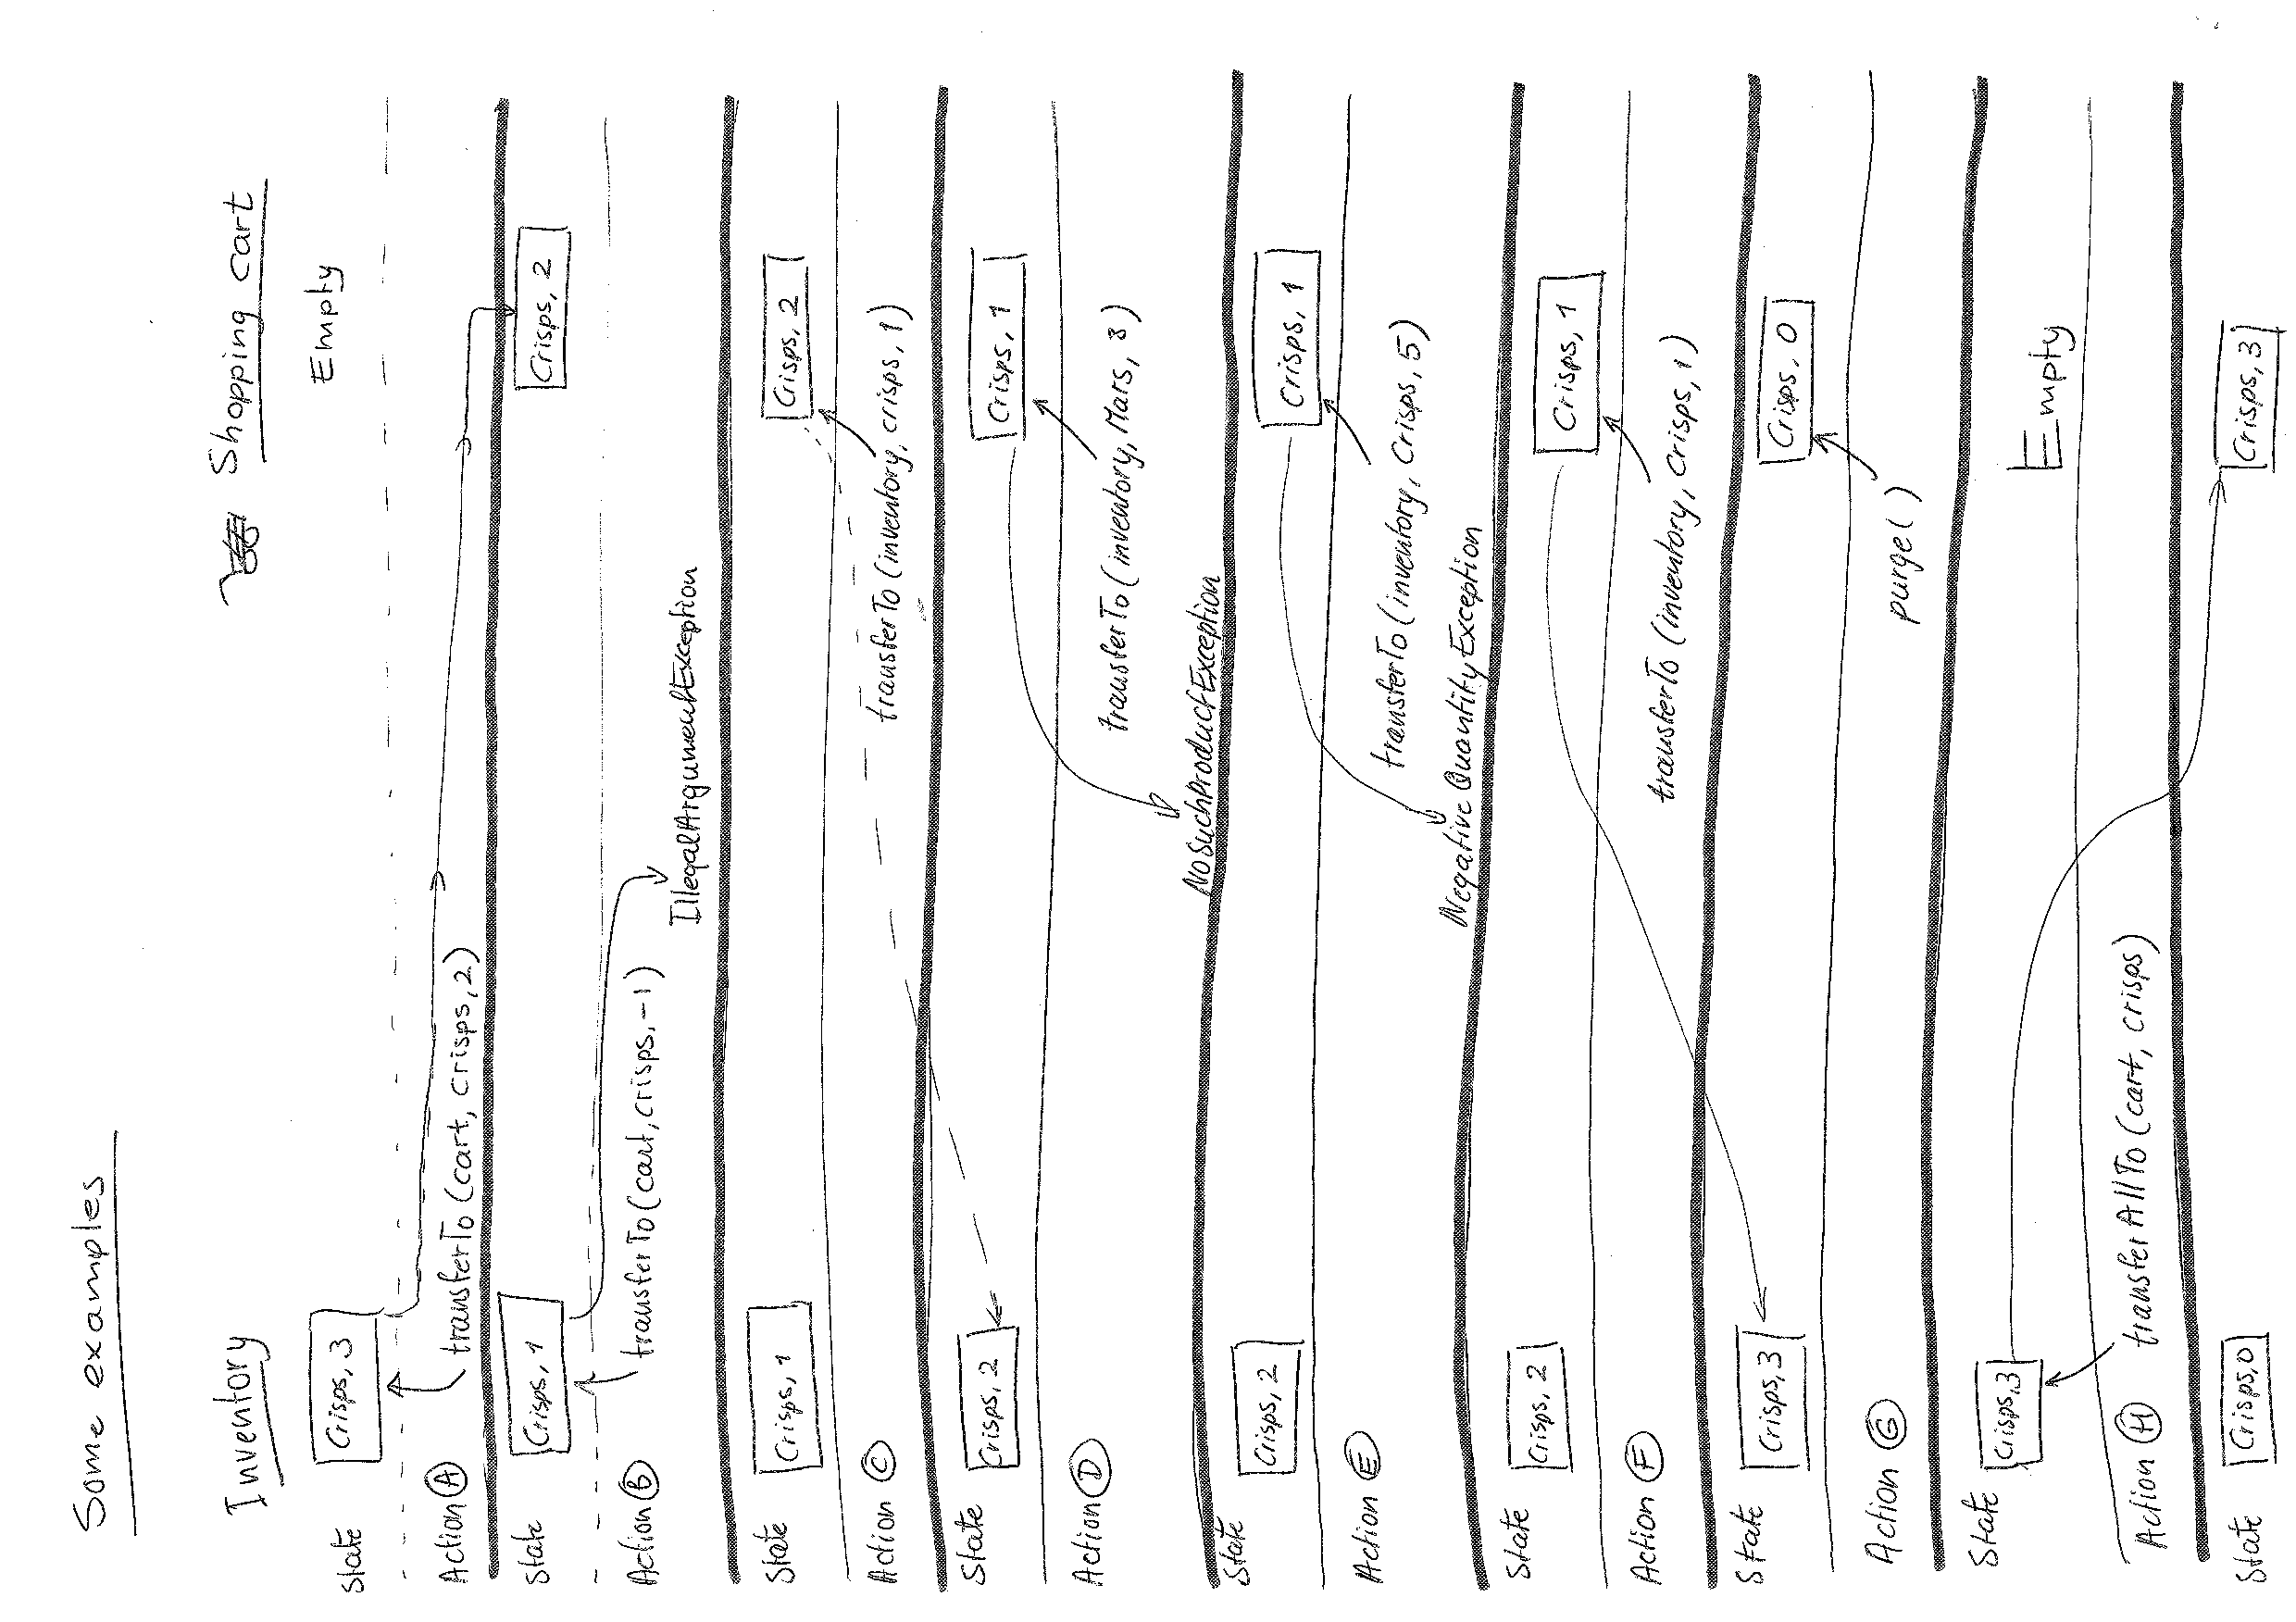
\includegraphics[angle=-90,width=\textwidth]{figures/assessment_napkin}
    \caption{\label{fig:napkin} ``Napkin'' design }
  \end{figure}
\end{center}


\section{Design}
\subsection{Simplifications}
For this assignment, some simplifications are applied, business wise.
\begin{itemize*}
\item There is no separate sales record, although accounting rules
  require it. However, such a \Code{Sales} record (product, qty, sales
  price and VATLevel) contains the same conceptual information as the
  \Code{InvoiceLine}. This is sufficient for the exercise.
\item Because of the above simplification, the model does not support
  returning goods. This is Okay, because we do not intend to sell this
  implementation anyway. We rather want to keep it stupid and secret
  at the same time.
\end{itemize*}

%\clearpage % let the napkin show up before the next paragraph.
\subsection{Architecture}
The \textit{project architecture} actually consists of two separate Netbeans projects. 
The idea behind this division into components is testability of
the business component called \textbf{webshopModel}.
The \textbf{webshop} is the web application which depends on this webshopModel. 

\subsection{Design of the product container}
Both cart and inventory can be considered as product containers,
meaning they contain tuples of (product,quantity). 
This tuple is modeled in a separate class \Code{ProductQuantity}. The 

The logical interaction between inventory and cart is a transfer of
(product,quantity) information. Note however, that these two containers
should never refer to the same (product,quantity) tuple.

The operation to \textit{take} products from a container is
\Code{take(Product,Quantity)}. This operation takes the specified amount from
the container and returns a \Code{ProductQuantity} tuple if successful. 
To \textit{put} products into the container we use the
\Code{ProductQuantity merge(ProductQuantity)} operation which \textit{adds to}
or \textit{sets} the current quantity to/with the new quantity. 

It is quite natural to use the result of the take operation as the parameter to the merge operation:
merge with the content of the cart what you took from the inventory.
 
Cart and inventory should behave differently when the amount is
set to zero by means of a \Code{transferToXXX()} operation. For the inventory, records
with zero quantity are allowed, whereas for the cart, records with zero
quantity should be deleted from the cart.

This matches the natural business situation that a quantity of zero in
an inventory leaves the shelve space intact, only empty.

In the cart however, the product, quantity tuple with quantity set to
zero has no meaning. 

To support this difference in behaviour, the ProductContainer has a method
called \Code{purge()} which removes any tuple having quantity equals
zero.

Therefor: In the business logic one should call \Code{cart.purge()}, but never \Code{inventory.purge()};
This difference between cart and inventory is expressed by the fact
that the classes \Code{Inventory} and \Code{Cart} both subclass
product container. See the class diagram in
figure~\ref{fig:classdiagram}.


In chapter~\ref{sec:realisation} you see that the project provides two
implementations for the persistence layer.

In the database persistence implementation , the inventory is backed by table
\texttt{inventory}, the cart by table \texttt{cart}.
